%!TEX root =../../../course-notes.tex
% ^ leave for LaTeXTools build functionality

\begin{applicationActivities}




\begin{activity}{5}
Why don't clouds fall out of the sky?
\begin{center}
\includegraphics[scale=0.2]{media/cloud.jpg}
\end{center}

\begin{enumerate}[(a)]
\item They are lighter than air
\item Wind keeps them from falling
\item Electrostatic charge
\item They do fall, just very slowly
\end{enumerate}
\end{activity}

\begin{activity}{5}
List all of the forces acting on a tiny droplet of water falling from the sky.
\end{activity}

\begin{activity}{5}
Tiny droplets of water obey \term{Stoke's law}, which says that air resistance is proportional to (the magnitude of) velocity.
\begin{itemize}
\item Let \(v\) be the velocity of a droplet of water (positive for upward, negative for downward).
\item Let \(g>0\) be the magnitude of acceleration due to gravity and \(b>0\) be another positive constant.
\end{itemize}
%Assume that the only forces acting on a falling droplet of water are gravity and air resistance.
\vfill
Apply Newton's second law (force \(=\) mass \(\times\) acceleration) 
to determine which of the following
\term{ordinary differential equations (ODEs)} models the velocity of a falling droplet of water. 
\vfill
\begin{enumerate}[(a)]
\item \(v'=g-v\)
\item \(v'=g+v\)
\item \(mv'=-mg-bv\)
\item \(mv'=-mg+bv\)
\end{enumerate}
\end{activity}

\begin{observation}
The modeling equation
\[mv'=-mg-bv\]
may be obtained by splitting the total force into gravity and air resistance:
\[F=F_g+F_r\]

Then \(F=ma=mv'\) and \(F_g=m(-g)=-mg\) are the result of Newton's second law,
and \(F_r=-bv\) holds because it should be (a) in the opposite direction of velocity 
and (b) a constant multiple of velocity.

\vfill

Note that this equation may be rearranged as follows to group \(v\)
and its derivative \(v'\) together on the left-hand side:

\[v'+\left(\frac{b}{m}\right)v=-g\]
\end{observation}

\begin{definition}
A \term{first order constant coefficient} differential equation can be written in the form
\[y^\prime+by=f(x),\]
or equivalently,
\[\frac{dy}{dx} +by=f(x).\]
We will use both notations interchangeably.
\vfill
Here, \term{first order} refers to the fact that the highest derivative we see is the first derivative of \(y\).
\end{definition}

\begin{observation}
Consider the differential equation \(y'=y\).

A useful way to visualize a first order differential equation is by a \term{slope field}


\begin{center}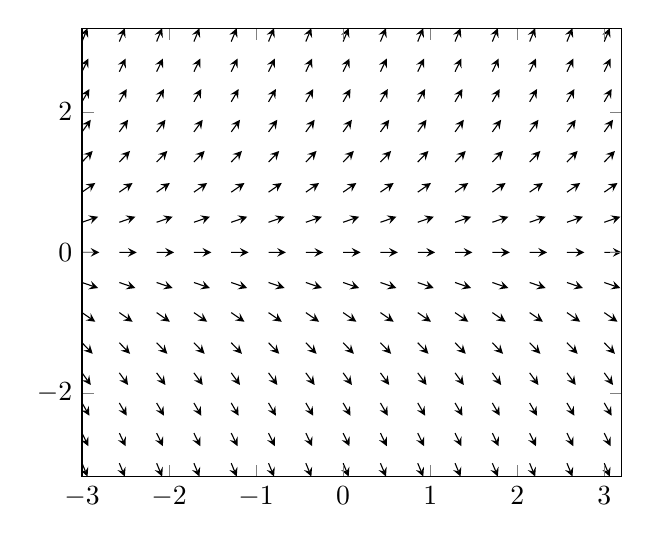
\begin{tikzpicture}
    \begin{axis}[
        domain=-3:3,
        view={0}{90},
        axis background/.style={fill=white},
    ]
        \addplot3[black,
            quiver={
             u={1/(sqrt(1 + (y)^2))},
             v={(y)/(sqrt(1 + (y)^2))},
             scale arrows=0.2,
            },
            -stealth,samples=15]
                {exp(-x) - 1/2*sin(x) - 1/2*cos(x)};
        %%KAWWWWWWW
        %% Here be some points added to the swoopy loop vector fieldamagigs
        %\addplot[mark=*] coordinates {(-1,2)}; % Obvious ordered pair for lococation
        %\addplot[mark=*] coordinates {(-1,-2)};
    \end{axis}
\end{tikzpicture}\end{center}
Each arrow represents the slope of a solution \term{trajectory} through that point.
\end{observation}

\begin{activity}{5}
Consider the differential equation \(y'=y\) with slope field below.

\begin{center}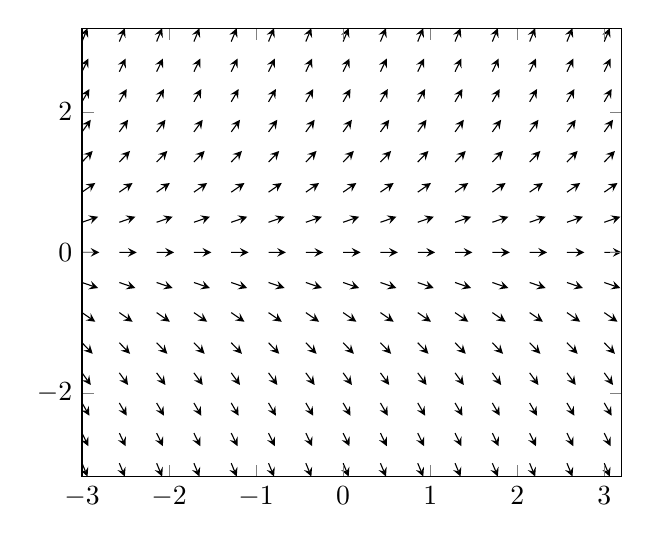
\begin{tikzpicture}
    \begin{axis}[
        domain=-3:3,
        view={0}{90},
        axis background/.style={fill=white},
    ]
        \addplot3[black,
            quiver={
             u={1/(sqrt(1 + (y)^2))},
             v={(y)/(sqrt(1 + (y)^2))},
             scale arrows=0.2,
            },
            -stealth,samples=15]
                {exp(-x) - 1/2*sin(x) - 1/2*cos(x)};
     \end{axis}
\end{tikzpicture}\end{center}
\begin{subactivity}
Draw a trajectory through the point \((0,1)\).
\end{subactivity}
\begin{subactivity}
Draw a trajectory through the point \((-1,-1)\).
\end{subactivity}
\end{activity}


\begin{activity}{15}
Consider the differential equation \(y^\prime=y\).
\begin{subactivity}
Find a solution to \(y^{\prime}=y\).
\end{subactivity}
\begin{subactivity}
Modify this solution to write an expression describing \textbf{all} solutions to \(y^{\prime}=y\).
\end{subactivity}
\end{activity}

\begin{definition}
A differential equation will have many solutions.
Each individual solution is said to be a \term{particular solution},
while the \term{general solution} encompasses \textbf{all} of these by using 
parameters such as \(C,k,c_0,c_1\) and so on. For example:

\begin{itemize}
\item The general solution to the differential equation \(y'=2x-3\) is \(y=x^2-3x+C\) (as done in
Calculus courses).
\item The general solution for \(y'=y\) is \(y=ke^x\) (as done in the previous activity). 
\end{itemize}

\end{definition}


\begin{activity}{15}
Adapt the general solution \(y=ke^x\) for \(y^\prime=y\) to find general solutions for
the following differential equations.
\begin{subactivity}
Solve \(y^{\prime}=2y\).
\end{subactivity}
\begin{subactivity}
Solve \(y^{\prime}=y+2\).
\end{subactivity}
\end{activity}

\begin{activity}{15}
Find the solution for \(y'=y+2\) directly.
\vfill
\textbf{Simple idea:} Since \(y_0=e^x\) was a particular solution of \(y'=y\), 
we guess that a particular solution for \(y'=y+2\) is of the form \(y_p =  v e^x\) 
for some \textbf{function} \(v(x)\). 
\vfill
\begin{subactivity}
Use the Product Rule to find \(y_p'=\frac{d}{dx}[ve^x]\).
\end{subactivity}
\begin{subactivity}
Substitute \(y_p\) and \(y_p'\) into the equation \(y'=y+2\).
\end{subactivity}
\begin{subactivity}
Solve for \(v'\), and integrate to find \(v\).
\end{subactivity}
\begin{subactivity}
Find \(y_p\).
\end{subactivity}
\end{activity}

\begin{observation}
The technique outlined in the previous activity is called \term{variation of parameters}.  
If \(y_0\) is a particular solution of the \term{homogeneous} equation, 
assume that a particular solution of the 
\term{non-homogeneous} equation has the form \(y_p = v y_0\), and then determine what \(v\) must be. 

\vfill

\textbf{Example: }
\begin{align*}
y'+3y = 0 & & \text{homogeneous} \\
y'+3y = x & & \text{non-homogeneous}
\end{align*}

Note that each term of the homogeneous equation includes \(y\) or it derivatives.
\end{observation}

\begin{activity}{20}
Solve \(y'=x-3y\) by first solving its corresponding homogeneous equation and using
variation of parameters: 
\begin{align*}
y'+3y = 0 & & \text{homogeneous} \\
y'+3y = x & & \text{non-homogeneous}
\end{align*}
\begin{subactivity}
Modify \(e^x\) to find the general solution \(y_h\) for the homogeneous equation.
\end{subactivity}
\begin{subactivity}
Choose a particular solution \(y_0\) for the homogeneous equation, and
assume \(y_p = v y_0 \) is a particular solution of the non-homogeneous equation for some \textbf{function} \(v\).
Substitute \(y_p\) into non-homogeneous equation and simplify.
\end{subactivity}
\begin{subactivity}
Determine \(v\), and then determine \(y_p\).
\end{subactivity}
\end{activity}

\begin{observation}
Since \(y_h=ke^{-3x}\) was the general solution of \(y'+3y=0\), 
and \(y_p = \frac{x}{3}-\frac{1}{9}\) is a particular solution of \(y'+3y=x\), 
\[y=y_h+y_p = \left(ke^{-3x}\right)+\left(\frac{x}{3}-\frac{1}{9}\right)\]
is a solution to \(y'+3y=x\):

\vfill

\[\frac{d}{dx}[y_h+y_p]+3(y_h+y_p)=(y_h'+3y_h)+(y_p'+3y_p)=0+x=x\]
\end{observation}

\begin{fact}
Let \(a\) be a constant real number.
Every constant coefficient first order ODE
\[y'+ay=f(x)\]
has the general solution
\[y=y_h+y_p\]
where \(y_h\) is the general solution to the homogeneous equation \(y'+ay=0\)
and \(y_p\) is a particular solution to \(y'+ay=f(t)\).
\end{fact}

\begin{activity}{15}
Find the general solution to \(y'=2y+x+1\) using variation of parameters:

\vfill

\begin{itemize}
\item Write the homogeneous equation and find its general solution \(y_h\).
\item Use a particular solution \(y_0\) for the homogeneous equation to find a particular solution
      \(y_p=vy_0\) for the original equation.
\item Then \(y=y_h+y_p\) gives the general solution to the equation.
\end{itemize}
\end{activity}

\end{applicationActivities}
